%!TEX root = ../thesis.tex
%3-Direct-Spectral-Recovery
% Shift and subtract Method
% Calculation of planet RV
% Simulation of spectral recovery
% RV difference effect on amplitude of signal simulation
% Chi squared method of model plus stellar at different RVs? technique
% Limitations?
% Future Prospects
% CRIRES+, JWST
% Calculation of exposure time required etc?


\chapter{Direct Spectral Recovery}  % Main chapter title
\label{cha:direct_recovery}
%----------------------------------------------------------------------------------------
%	SECTION 1
%----------------------------------------------------------------------------------------
There many different techniques to disentangle the spectra of binary objects. In this chapter we focus on applying a direct subtraction method to near-infrared (\nir{}) spectra of FGK stars with Brown Dwarf (BD) companions. The data used was obtained with the CRIRES instrument in 2012, (before it was removed its upgrade) with the purpose to apply this technique specifically. A level of trust was placed in the quality of the observations, which was misplaced.
We start this chapter by explaining the direct subtraction technique. We will then explain the motivation for the specific targets observed. We will detail the observations, showing each the orbital position of each observation. After revealing the insufficient signal from this technique we will explore the limitations of these observations followed by some simulated results.

\section{Motivation}


Motivation section

Why this technique and not others.
- separation of components
- direct imaging (cant separate)


Find direct imaging limitations ---



\section{Differential subtraction (new)}
\label{sec:spec_diff}
{\red This is the summary in the paper}
The observations were gathered having in mind the application of a differential subtraction method~\citep[e.g.][]{ferluga_separating_1997, kostogryz_spectral_2013} to detect the spectra of the faint BD companions. In short, we Doppler shift each observation to the rest frame of the host star and then mutually subtract the spectra from pairs of observations to cancel out the spectra of the brighter host star. The residuals from this method should contain two copies of the faint companion, subtracted from each other with a radial velocity offset \(\Delta RV\) between them. This RV offset, if detectable, would allow the mass ratio to be determined and hence the companion mass.

Due to the poorly separated observation times relative to the long orbital periods, this method was revealed to be inappropriate for these observations as the RV separation of the companion spectra between observations (\(\le 2.3\)\kmps{}) is significantly smaller than the FWHM (full width half maximum) of individual spectral lines (\(\sim\)6\kmps{} at \(\rm R=50\,000\)).  The small separation of the companion causes the lines of the companion to also mutually cancel, severely reducing the residual signal to well below the available noise level. The requirement of well separated RVs for the companion spectra was clearly stated in the original proposal but was not satisfied when the observations were obtained\footnote{see Sect.~\ref{subsubsec:differential-schedualing} for more details}. {\red{} The very large orbital periods of some of the targets would not produce a sufficient RV signal during one semester. This was a possible oversight during the proposal stage.} The largest estimated companion \(\Delta RV\) separation between the observations of each target is provided in the seventh column of Table~\ref{tab:estimated_rv}. Radial velocity constraints are also valid for other studies such as the detection of reflected light from exoplanets~\cite{martins_evidence_2015}.

Despite these problems, we still tried to apply the method to our data. Given the negative result, however, we decided to move this section to Appendix~\ref{sec:direct-subtraction}, where we describe the method and some exploratory results that may be useful for future studies.



\section{Direct Subtraction Method}
\label{sec:direct-subtraction}
Here we outline the direct subtraction method used, which is similar to previous works~\citep{ferluga_separating_1997,kostogryz_spectral_2013}. Assuming that the instrumental profile and atmospheric absorption are dealt with appropriately, the spectrum received from the host-companion pair is given by the superposition of two spectral components (\(J_{1} \), \(J_{2} \)), where \(\lambda-v\) represents the Doppler shift \(\lambda(1-v/c)\) by velocity \(v\).
\begin{equation}
\textrm{I}(\lambda) = \textrm{J}_{1}(\lambda - v_{1}) + \textrm{J}_{2}(\lambda - v_{2})
\end{equation}
or shifted to the host stars rest frame,
\begin{equation}
\textrm{I}(\lambda + v_{1}) = \textrm{J}_{1}(\lambda) + \textrm{J}_{2}(\lambda - v_{2} + v_{1})
\end{equation}
Here, the subscripts 1 and 2 indicate the spectrum of the host and companion respectively, and \(\lambda\) represents the wavelength of the spectra.
The spectra of the host star (\(\textrm{J}_{1} \)) is removed though the mutual subtraction of the host spectrum from two separate observations, denoted with subscripts \(a\) and \(b\), correcting for RV motion of the host star.
\begin{align}
S(\lambda) &= \textrm{I}_{a}(\lambda + v_{1a}) - \textrm{I}_{b}(\lambda + v_{1b}) \nonumber \\
&= \textrm{J}_{2}(\lambda - v_{2a} + v_{1a}) - \textrm{J}_{2}(\lambda - v_{2b}  + v_{1b}) \nonumber \\
%  &= \textrm{J}_{2}(\lambda - v_{2a}) - \textrm{J}_{2}(\lambda - v_{2b} - v_{1a} + v_{1b}) \nonumber \\
S(\lambda + v_{2a}) &= \textrm{J}_{2}(\lambda) - \textrm{J}_{2}(\lambda + \Delta RV )  \label{eqn:sprofile}
\end{align}
where,
\begin{equation}
\Delta RV = v_{2a} - v_{2b} - v_{1a} + v_{1b} \label{eqn:k}
\end{equation}

is the actual RV difference (\(\Delta RV \)) between the two companion spectra.

The resulting differential spectra, dubbed \emph{s-profile} by~\citet{ferluga_separating_1997}, is composed of just the companion spectra, shifted and subtracted from itself.

From binary dynamics~\citep[e.g.][]{murray_keplerian_2010} the RV amplitudes of the host and companion are related through the mass ratio, \(q \), while having an opposite sign.
\begin{align}
v_{2}  &= -\textrm{q} * v_{1} \label{eqn:q_relation}
\end{align}
This equation was used to calculate the expected companion RV for each observation in Table~\ref{tab:observations}.

We can simplify Eq.~\ref{eqn:k} by expressing it in terms of the host RV and mass ratio,
\begin{align}
k &= -q v_{1a} + q v_{1b} + v_{1a} - v_{1b} \nonumber \\
&= (1 - \textrm{q})(v_{1a} - v_{1b}). \label{eqn:k_simplified}
\end{align}
If we are able to determine the \(\Delta RV\) between the the companion spectra, k, from the s-profile~\citep[see ][]{ferluga_separating_1997} then we can determine the mass ratio of the system, q, thereby constraining the mass of the companion. The values \(v_{1a}\) and \(v_{1b}\) are calculated from the orbital parameters of the system and are the same values already used to shift and mutually cancel the host spectrum.

This method is very similar to~\citet{kostogryz_spectral_2013} except that they focus on M-dwarfs host stars with the observations taken at the extrema, in which the companion lines are well separated.




\subsection{The Data}

\subsection{CRIRES data}
\label{subsec:CRIRES}
Observations were performed with the CRIRES instrument~\citep{kaeufl_crires_2004} configured to observe a narrow wavelength domain of the K-band between 2120--2160\nm{} using the Ks and the Hx5e-2 filters. The slit width of \(0.4\sec\) resulted in an instrumental resolving power of \(\rm R=50\,000\), with no adaptive optics to ensure that the slit was entirely covered by each target. This prevents strong slit illumination variations that could change the shape of spectral lines.

The observations were performed in service mode during period 89 with run ID.~089.C-0977(A) between April and August 2012. An observation is composed of 8 individual spectra with an integration time of 180 seconds, observed in the ABBAABBA nod cycle pattern to obtain a high (>100) signal-to-noise when combined. The list of observations obtained with CRIRES are provided in Table~\ref{tab:observations}.

%!TEX root = ../nir_companions.tex

% Table of observations
\begin{table*}
    \small
            \centering  
           \begin{threeparttable}[b]
     
            \caption{Details about the each CRIRES observation. {\rd{} The time, settings, number of artefacts removed, the SNR obtained and the predicted orbital state of each system are provided.}}
            %\begin{tabular}{l c c c c cl cl r@{.}l r@{.}l r@{.}l}
            \begin{tabular}{l c c c c c c r@{.}l r@{.}l r@{.}l}
                \toprule
                Object & Obs. \# & Start date  & Filter & Airmass  & Artefacts & SNR & \multicolumn{2}{c}{\(RV_1\)} & \multicolumn{2}{c}{\(RV_2\)} & \multicolumn{2}{c}{\(rv_2\)}  \\  % & \(Date \)
                &   & (yyyy-mm-dd hh:mm:ss)  &  & (at start) & {\rd / 32} & & \multicolumn{2}{c}{kms\(^{-1}\)} & \multicolumn{2}{c}{kms\(^{-1}\)} & \multicolumn{2}{c}{kms\(^{-1}\)}\\ % data ref    % & (JD\(^{\star} \))
                \midrule
                {HD 4747}   & 1 & 2012-07-06 07:36:06 & Ks     	      & 1.25  	  & 7 & 340 & $-$0    & 219 & $-$0  & 154 & 0&065 \\ %-1      & 2456114.81674
                {HD 162020} & 1 & 2012-07-04 06:23:22 & Ks     		& 1.30 		& 2 & 127 & $-$28  & 760 & 50 & 785\tnote{a}  & 79&545\tnote{a} \\ %-1      & 2456112.76624
                {HD 162020} & 2 & 2012-07-04 06:57:48 & Ks     		& 1.44  	& 2 & 128 & $-$28  & 717 & 48 & 440\tnote{a} & 77&157\tnote{a} \\ %-2      & 2456112.79015
                {HD 167665} & 1 & 2012-07-28 05:00:53 & Hx5e-2 	& 1.24 		& 7 & 371 & 7         & 581 & 18 & 024\tnote{a} & 10&443\tnote{a} \\ %-1a     & 2456136.70895
                {HD 167665} & 2 & 2012-07-28 05:37:27 & Hx5e-2 	& 1.39  	& 4 & 374 & 7         & 581 & 18 & 025\tnote{a}  & 10&444\tnote{a} \\ %-1b     & 2456136.73434
                {HD 167665} & 3 & 2012-08-05 02:54:03 & Hx5e-2 	& 1.04  	& 4 & 358 & 7         & 575 & 18 & 163\tnote{a} & 10&588\tnote{a} \\ %-2      & 2456144.62087
                {HD 168443} & 1 & 2012-08-05 04:29:32 & Ks     		& 1.31 		& 2& 192 & $-$0   & 121 & 50 & 932\tnote{a,b}  & 51&053\tnote{a,b} \\ %-1      & 2456144.68718
                {HD 168443} & 2 & 2012-08-05 04:58:50 & Ks     		& 1.47 		& 4 & 190 & $-$0   & 121 & 51 & 189 \tnote{a,b} & 51&310\tnote{a,b} \\ %-2      & 2456144.70753
                {HD 202206} & 1 & 2012-07-12 06:54:44 & Ks     		& 1.01 		& 3& 189 & 14      & 843 & 12 & 992\tnote{b}  & -1&851 \\ %-1      & 2456120.78801
                {HD 202206} & 2 & 2012-07-13 05:41:40 & J       	  & 1.01 	  & 3 & 209 & 14      & 837 & 13 & 065\tnote{b}  & -1&772 \\ %-2      & 2456121.73727
                {HD 202206} & 3 & 2012-07-11 08:29:55 & Ks     		& 1.15		& 4& 180 & 14      & 849 & 12 & 920\tnote{b}  & -1&929 \\ %-3      & 2456119.85411
                {HD 211847} & 1 & 2012-07-06 07:02:57 & Ks     		& 1.07 		& 4& 272 & 6        & 613 & 7   & 171 & 0& 558\\ %-1      & 2456114.79372
                {HD 211847} & 2 & 2012-07-13 06:54:37 & Ks     		& 1.05 		& 5& 283 & 6        & 614 & 7   & 167 & 0&553 \\ %-2      & 2456121.78793
                {HD 30501}  & 1 & 2012-04-07 00:08:29 & Hx5e-2 	 & 1.60 	 & 3& 217 & 22      &  372 & 36 & 377 & 14&005 \\ %-1      & 2456024.50590
                {HD 30501}  & 2 & 2012-08-01 09:17:30 & Hx5e-2    & 1.42     & 10& 212 & 22      & 505 & 35  & 120 & 12&615 \\ %-2a     & 2456140.88716
                {HD 30501}  & 3 & 2012-08-02 08:47:30 & Hx5e-2 	 & 1.53 	 & 8& 237 & 22      & 507 &  35 & 102 & 12&595 \\ %-3      & 2456141.86633
                {HD 30501}  & 4 & 2012-08-06 09:42:07 & Ks     		 & 1.28 	 & 7& 235& 22      & 514 & 35 & 031 & 12&517 \\ %-2b     & 2456145.90426
                \bottomrule
                & & & & 
        \end{tabular}
        \label{tab:observations}
        \begin{tablenotes}
          \item  [a]{Maximum RV given \(\textrm{M}_2\sin{i}\) only.}
          \item  [b]{Largest mass companion only.}
        \end{tablenotes}
    \end{threeparttable}

\end{table*}







    \subsection{Estimating parameters of observations}
    To estimate the differential amplitude signal we estimated the expected parameters of the impact of the

    %!TEX root = ../thesis.tex
\begin{table*}
         \small
        \centering
       %\begin{threeparttable}[b]
        \caption{Estimated flux ratios given the companion mass (\(\textrm{M}_{2}\) or \(\textrm{M}_{2} \sin{i}\)) from Table~\ref{tab:orbitparams}.} 
        \begin{tabular}{l c c c c c c c}%[hb]
            \toprule
            & Host& Companion & Estimated & Estimated & \\  % 2017
            Companion & M\(_{K}\) & M\(_{K}\) & \(\rm F_{2}/F_{1} \) & \(\rm N_{2}/N_{1} \) (noise ratio) \\
            & & & \textit{K}-band & \\
            \midrule
            {HD 4747} & 3.82 & 14.17 & \(7\times10^{-5} \) & 76 \\  % 2017
            {HD 162020} & 4.10 & 23.36 & \(2\times10^{-8} \) & 1615 \\  %
            {HD 167665} & 2.60 & 13.21 & \(6\times10^{-5} \) & 105 \\  %  -- \(2\times10^{-5} \)  best case based on age rage.
            {HD 168443b} & 2.35 & 42.19 & \(1\times10^{-16} \) & \(1\times10^{8} \) \\ 
            {HD 168443c} & 2.35 & 29.55 & \(1\times10^{-11} \) & \(4\times10^{5} \) \\  %(c)
            {HD 202206}B & 3.04& 21.63 & \(4\times10^{-8} \) & 1586 \\  %(B)   % May2017
            {HD 202206}c & 3.04& 45.63 & \(9\times10^{-18}\) & \(2\times10^{7} \) \\  %(B)   % May2017
            {HD 211847}B & 3.50 & 8.40 & 0.011 & 14 \\  %B % 2017
            {HD 30501} & 3.96 & 10.38 & 0.003 & 27 \\
            \bottomrule& & 
        \end{tabular}
            \label{tab:estimated_flux_ratios}
 % \end{threeparttable}

\end{table*}
    %!TEX root = ../thesis.tex
\todo{Fix caption position here}
\begin{table*}
        \small
        \centering
       \begin{threeparttable}[b]
        \caption{Estimated orbital semi-amplitude and {RV} separation of the companion, given the companion mass (\(\textrm{M}_{2}\) or \(\textrm{M}_{2} \sin{i}\)) from \tref{tab:orbitparams} and observation times from \tref{tab:observations}.} 
       \begin{tabular}{l c c c c c c}%[hb]
           \toprule
           & Estimated & Estimated & & \\  % 2017
           Companion & \(\rm K_2\) & \(\Delta {RV}\) & Phase coverage\\
           & (\kmps{}) & (\mps{}) & (\%)\\
           \midrule
           {HD 4747} & -10.65 & -- & --\\  % 2017
           {HD 162020} & -98.92\tnote{a} & 2\,344.24 & 0.28\\  %
           {HD 167665} & -14.47\tnote{a} & 138.45 & 0.18\\  %  -- \(2\times10^{-5} \)  best case based on age rage.
           {HD 168443b} & -64.65\tnote{a}& 257.16 & 0.035\\ 
           {HD 168443c} & -18.05\tnote{a} & 0.95 & 0.001\\  %(c)
           {HD 202206}B & -6.79 & 145.17 & 0.74\\  %(B)   % May2017
           {HD 202206}c & -2.50 & 0.67 & 0.15\\  %(B)   % May2017
           {HD 211847}B & $-$1.85 & 3.88 & 0.09\\  %B % 2017
           {HD 30501} & -16.12 & 1\,346.46 & 5.8\\
           \bottomrule   
           \end{tabular}
            \label{tab:estimated_rv}
    \begin{tablenotes}
        \item[a] {Maximum \(K_2\) only given \(M_2 \sin{i}\)}
      \end{tablenotes}
  \end{threeparttable}

\end{table*}
    %!TEX root = ../thesis.tex
\begin{table*}
    %\tiny
    \small
    \centering
    \caption{Estimated flux ratios and semi-amplitude of the companion given the companion \(\textrm{M}_{2}/\textrm{M}_{2} \sin{i}\) from Table~\ref{tab:orbitparams}. The flux ratio \(F_{2}/F_{1} \) is calculated using the K-band magnitude difference of the host star to the Baraffe evolutionary model magnitude for the companion mass. The model ages used are those closest to host age value in Table~\ref{tab:starparams}.     The noise ratio is  calculated via \(N_{2}/N_{1} = \sqrt{2} \times\sqrt{F_{1}/F_{2}}\). The orbital properties are calculated using the orbital parameters given above along with the times of observations in Table~\ref{tab:observations}.} 
    \begin{tabular}{l c c c c c c c c}
        \toprule
        &  Estimated  & Estimated &  Estimated & Estimated &  &    \\  % 2017
        Host           & \(\rm F_{2}/F_{1} \)   & \(\rm N_{2}/N_{1} \) (noise ratio) & \(\rm K_2\) &   \(\Delta RV\) & Phase coverage \\
        & K-band     & & (kms\(^{-1}\)) & (ms\(^{-1}\)) & (\%) \\
        \midrule
        \object{HD 4747}        & \(3\times10^{-4} \)   & 76 &  -10.65 & -  &  -  \\  % 2017
        \object{HD 162020}   & \(7\times10^{-7} \)   & 1615  &  -98.92\tablefootmark{a} &  2344.24     & 0.28~~  \\  %
        \object{HD 167665}    & \(2\times10^{-4} \)   &  105    &  -14.47\tablefootmark{a}   &   138.45     & 0.18~~  \\  %  -- \(2\times10^{-5} \)  best case based on age rage.
        \object{HD 168443b} & \(1\times10^{-16} \)  &    \(1\times10^{8} \)   &  -64.65\tablefootmark{a} &   257.16   & 0.035 \\ 
        \object{HD 168443c} &  \(1\times10^{-11} \)  &   \(4\times10^{5} \)     &  -18.05\tablefootmark{a}  &   0.95   &  0.001 \\  %(c)
        \object{HD 202206}B  & \(8\times10^{-7} \)  &   1586 &  -6.79 & 145.17   & 0.74~  \\  %(B)   % May2017
        \object{HD 202206}c  &  \(5\times10^{-15}\)   &     \(2\times10^{7} \) &   -2.50     &   0.67     &  0.15~  \\  %(B)   % May2017
        \object{HD 211847}B  &  0.01 &  14   & $-$1.85 & 3.88   & 0.09~  \\  %B % 2017
        \object{HD 30501}      &  0.002  &  27  &  -16.12    &  1346.46      & 5.8~~  \\
        \bottomrule
    \end{tabular}\\
    \tablefoot{
        \tablefoottext{a}{Maxium \(K_2\) only given \(M_2 \sin{i}\)}
    }
    \label{tab:flux_table}
\end{table*}    % THIS is the old table.

    \subsection{Results of spectral differential analysis}

    \label{appendix:A2}
    We applied the spectral differential procedure outlined above on the wavelength-calibrated and telluric-corrected CRIRES observations. The spectra were corrected for Earth's barycentric RV using the \emph{helcor} PyAstronomy\footnote{https://pyastronomy.readthedocs.io} function ported from the REDUCE IDL package (See~\citet[][]{piskunov_new_2002}) and Doppler shifted to the rest frame velocity of the system. The spectra were then subtracted from each other and analysd as described above.

    It is necessary to have a consistent instrumental setup~\citet{ferluga_separating_1997}, to avoid introducing extra instrumental effects (e.g.\ slit-width and/or filters) into the spectral differentials and to always observe the same wavelength range and maximize the information to be extracted. In our case, the second observation of {HD 202206} and fourth of {HD 30501} were taken with different filters compared to the other observations. Therefore, these two observations could not be used for this differential analysis. As noted in~\citep{hadrava_disentangling_2009}, any spectral differences in the filters would add extra unknown signal/noise making it harder to disentangle the faint spectral differences.


    \begin{figure}
        \centering
        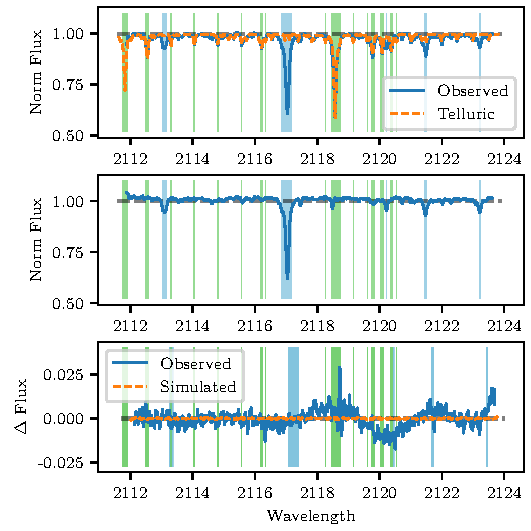
\includegraphics[width=0.8\hsize]{figures/direct-recovery/differential.pdf}\\
        \caption{ (Top) A reduced CRIRES observation of {HD 30501} (blue) for detector 1 between 2112--2124\nm{} along with the tapas telluric absorption model ({orange} dashed) used for the wavelength calibration and telluric correction. (Middle) The telluric corrected spectra. (Bottom) ({blue}) Differential spectra for {HD 30501} between observations 1 and 3. ({orange} dashed) Simulated ``perfect'' differential using PHOENIX-ACES spectra with parameters \(T_{\textrm{eff}} = 2500~K \), \(\rm logg=5.0\), and \(\rm [Fe/H]=0.0 \), with the same \(\Delta RV\) as the observations. The shaded regions indicate where the telluric {green} and host star {blue} spectra are > 4\% deep.}
        \label{fig:spectral_example}
    \end{figure}

    We performed the differential analysis for all targets but only show our most favourable case here, {HD 30501}, because it is the second largest companion in our sample at \(\rm 90~M_{Jup}\) and also has the second largest RV separation between observations. The differential spectra recovered for {HD 30501} is shown at the bottom panel of Fig.~\ref{fig:spectral_example}. The presence of deep (\(>4\% \)) stellar and telluric lines in the original spectrum is shaded by the blue and green regions respectively. This indicates that the features of the differential spectrum near these shaded regions are likely due to imperfect telluric correction and host mutual cancellation.
    The mutual cancellation of the stellar host works well for the \(\sim40\%\) deep line near 2117~nm, being completely removed, but it does not do so well for the smaller \(\sim10\%\) deep line around 2121.5~nm. The residual for the large \(\sim40\%\) deep telluric line near 2118.5\nm{} is quite prominent. There is also a wider residual due to three neighbouring lines \(\sim10\%\) deep around 2120\nm{} which cause features in the differential spectrum. One possible explanation is that the continuum normalization near 2120\nm{} was influenced by this grouping of lines.

    To understand the observed differential signal we simulated a differential spectrum of {HD 30501} using a synthetic PHOENIX-ACES spectra with parameters \(T_{\textrm{eff}} = 2500~K \), \(\rm logg=5.0 \), and \(\rm [Fe/H]=0.0 \), with a RV offset estimated from the observation times. These parameters represent an estimated companion \(T_{\textrm{eff}}\) with the metallicity and logg similar to the host (closest grid model). The model spectra were convolved to \(\rm R=50\,000 \), continuum normalized and scaled by the estimated flux ratio of the companion. We do not include any synthetic host or telluric spectra and as such simulate the differential result of a ``perfect'' host cancellation with no telluric contamination present. This is the ideal-case scenario, and we stress that it is impossible to simulate the effect of improper telluric correction in a meaningful way. When comparing the simulated and observed differential in the bottom panel of Fig.~\ref{fig:spectral_example}, there is a striking amplitude difference. The orange-dashed line of the simulated differential spectrum amplitude is of a much smaller scale than the observed differential. This demonstrates that the amplitude of the differential signal we are trying to detect is much smaller than the residuals created by this differential technique.

    The amplitude of the differential signal is lower than we expected due to the very low \(\Delta RV\) between the observation pairs. The maximum \(\Delta RV\) between observation pairs, for the observations investigated in this work, are provided in Table~\ref{tab:estimated_rv}. {\red{} There is no \(\Delta RV\) for {HD 4747} as there was only a single observation. We also provide the phase coverage for our targets. We calculate this as the ratio of time between the observed pairs and the orbital period, and show that the fraction of the orbit covered is very small, all except one covering less than 1 percent of the orbit.}

    In our best case, {HD 30501}, the \(\Delta RV\) of the companion between observations is 1.346\kmps{}. For comparison, a single Gaussian absorption line, to be shifted by \(\Delta\lambda = \rm FWHM\) would need a \(\Delta RV\) of \(v_{\textrm{FWHM}} = c/R =~\sim6\)\kmps{}. Since the \(\Delta RV\) are shifted by a smaller value than the FWHM, the spectral lines of the reconstruction mutually cancel themselves, diminishing the amplitude of the differential signal significantly. As the companion spectra are already faint (with a flux ratio at the percent level) the differential signal is not detectable within these observations and noise level.
    When the \(\Delta RV\) of the companion is smaller than the FWHM of a line there is a mutual subtraction of the companion spectra, diminishing the detected amplitude of the differential signal, and removing the ability to detect the companions using this method. Observations need to be spaced further apart in time/phase to achieve a larger \(\Delta RV\) separation and increase the amplitude of the differential. Of course once there is a separation there will be complex interactions between neighbouring lines that need to be accounted for.

    \subsection{Relative differential amplitude}
    To probe this issue further we investigated how the amplitude of the differential signal changed with \(\Delta RV \). Taking the same PHOENIX-ACES spectra (\(T_{\textrm{eff}} = 2500~K \), \(\rm logg=5.0 \), \(\rm [Fe/H]=0.0 \)), we computed differential spectra for a range of \(\Delta RV\)s between \(\pm10\)\kmps{}. Figure~\ref{fig:diff_amp} shows how the relative amplitude of the differential spectrum in the wavelength range 2110--2123\nm{} (detector 1 of our CRIRES observations) changed as the spectra are offset. At each RV step we take the maximum absolute differential value found. These are then normalized by the median value outside of the line FWHM (dashed vertical lines), between \(\pm(7-10)\)\kmps{}, to give a relative differential amplitude, independent from the depth of a specific line. For comparison we also show the relative amplitude of the differential spectrum for a single Gaussian and single Lorentzian line when Doppler shifted by the same \(\Delta RV \)s. The shape of these results is also consistent with the analytical form of the differential spectra~\citet[][eqn.~A.1]{ferluga_separating_1997}.

    At a \(\Delta RV\) difference of zero, spectral lines of the companion completely cancel each other out, resulting in zero amplitude. As the RV separation increases, the individual lines stop cancelling themselves until a maximum differential amplitude is achieved when the lines are fully separated from themselves (equal to the line depth).

    The two solid vertical lines in Fig.~\ref{fig:diff_amp} indicate the estimated \(\Delta \textrm{RV}\)=1.346\kmps{} separation for our best target, {HD 30501} from Table~\ref{tab:estimated_rv}, given known orbital parameters and the observation times. This shows that our differentials have severely reduced amplitude, \(<20\%\) relative to well separated individual lines. As the companion spectra are faint and in combination with a host star at 1\% flux ratio the >80\% extra reduction in signal amplitude makes this detection impossible with these observations.

    In the synthetic spectrum (and of course real spectra) neighbouring spectral lines begin to interfere, leading to an impact on the measured relative amplitude. We suspect that the interaction of neighbouring lines is one possible cause for the difference between the theoretical and simulated shape between 2 and 6\kmps{}. Beyond the RV range present the amplitude becomes complicated due to neighbouring line interaction, but as the \(\Delta RV\) for all our spectra fall well short of this region we did not investigate this further.


%%%%%%%%%%%%%%%%%%%
\subsection{Results of spectral differential analysis}

\label{appendix:A2}
We applied the spectral differential procedure outlined above on the wavelength-calibrated and telluric-corrected CRIRES observations. The spectra were corrected for Earth's barycentric RV using the \emph{helcor} PyAstronomy\footnote{https://pyastronomy.readthedocs.io} function ported from the REDUCE IDL package (See~\citet[][]{piskunov_new_2002}) and Doppler shifted to the rest frame velocity of the system. The spectra were then subtracted from each other and analysed as described above.

It is necessary to have a consistent instrumental setup~\citet{ferluga_separating_1997}, to avoid introducing extra instrumental effects (e.g. slit-width and/or filters) into the spectral differentials and to always observe the same wavelength range and maximize the information to be extracted. In our case, the second observation of \object{HD 202206} and fourth of \object{HD 30501} were taken with different filters compared to the other observations. Therefore, these two observations could not be used for this differential analysis. As noted in~\citep{hadrava_disentangling_2009}, any spectral differences in the filters would add extra unknown signal/noise making it harder to disentangle the faint spectral differences.


\begin{figure}
	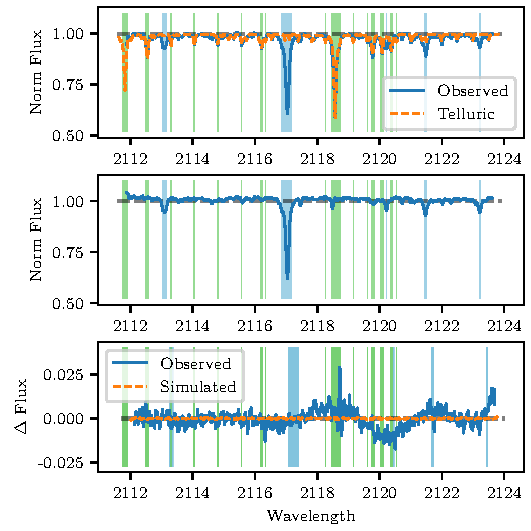
\includegraphics[width=\hsize]{figures/direct-recovery/differential.pdf}\\
	\caption{ (Top) A reduced CRIRES observation of \object{HD 30501} (blue) for detector 1 between 2112--2124\nm{} along with the tapas telluric absorption model ({orange} dashed) used for the wavelength calibration and telluric correction. (Middle) The telluric corrected spectra. (Bottom) ({blue}) Differential spectra for \object{HD 30501} between observations 1 and 3. ({orange} dashed) Simulated ``perfect'' differential using PHOENIX-ACES spectra with parameters \(T_{\textrm{eff}} = 2500~K \), \(\rm logg=5.0\), and \(\rm [Fe/H]=0.0 \), with the same \(\Delta RV\) as the observations. The shaded regions indicate where the telluric {green} and host star {blue} spectra are > 4\%  deep.}
	\label{fig:spectral_example}
\end{figure}


We performed the differential analysis for all targets but only show our most favourable case here, \object{HD 30501}, because it is the second largest companion in our sample at \(\rm 90~M_{Jup}\) and also has the second largest RV separation between observations. The differential spectra recovered for \object{HD 30501} is shown at the bottom panel of Fig.~\ref{fig:spectral_example}. The presence of deep (\(>4\% \)) stellar and telluric lines in the original spectrum is shaded by the blue and green regions respectively. This indicates that the features of the differential spectrum near these shaded regions are likely due to imperfect telluric correction and host mutual cancellation.
The mutual cancellation of the stellar host works well for the \(\sim40\%\) deep line near 2117~nm, being completely removed, but it does not do so well for the smaller \(\sim10\%\) deep line around 2121.5~nm. The residual for the large \(\sim40\%\) deep telluric line near 2118.5\nm{} is quite prominent. There is also a wider residual due to three neighbouring lines \(\sim10\%\) deep around 2120\nm{} which cause features in the differential spectrum. One possible explanation is that the continuum normalization near 2120\nm{} was influenced by this grouping of lines.

To understand the observed differential signal we simulated a differential spectrum of \object{HD 30501} using a synthetic PHOENIX-ACES spectra with parameters \(T_{\textrm{eff}} = 2500~K \), \(\rm logg=5.0 \), and \(\rm [Fe/H]=0.0 \), with a RV offset estimated from the observation times. These parameters represent an estimated companion \(T_{\textrm{eff}}\) with the metallicity and logg similar to the host (closest grid model). The model spectra were convolved to \(\rm R=50\,000 \), continuum normalized and scaled by the estimated flux ratio of the companion. We do not include any synthetic host or telluric spectra and as such simulate the differential result of a ``perfect'' host cancellation with no telluric contamination present. This is the ideal-case scenario, and we stress that it is impossible to simulate the effect of improper telluric correction in a meaningful way. When comparing the simulated and observed differential in the bottom panel of Fig.~\ref{fig:spectral_example}, there is a striking amplitude difference. The orange-dashed line of the simulated differential spectrum amplitude is of a much smaller scale than the observed differential. This demonstrates that the amplitude of the differential signal we are trying to detect is much smaller than the residuals created by this differential technique.

The amplitude of the differential signal is lower than we expected due to the very low \(\Delta RV\) between the observation pairs. The maximum \(\Delta RV\) observed between pairs of all targets is provided in Table~\ref{tab:estimated_fluxratio}.
In our best case, \object{HD 30501},  the \(\Delta RV\) of the companion between observations is 1.346\kmps{}. For comparison, a single Gaussian absorption line, to be shifted by \(\Delta\lambda = \rm FWHM\) would need a \(\Delta RV\) of \(v_{\textrm{FWHM}} = c/R =~\sim6\)\kmps{}. Since the \(\Delta RV\) are shifted by a smaller value than the FWHM, the spectral lines of the reconstruction mutually cancel themselves, diminishing the amplitude of the differential signal significantly. As the companion spectra are already faint (with a flux ratio at the percent level) the differential signal is not detectable within these observations and noise level.
When the \(\Delta RV\) of the companion is smaller than the FWHM of a line there is a mutual subtraction of the companion spectra, diminishing the detected amplitude of the differential signal, and removing the ability to detect the companions using this method. Observations need to be spaced further apart in time/phase to achieve a larger \(\Delta RV\) separation and increase the amplitude of the differential. Of course once there is a separation there will be complex interactions between neighbouring lines that need to be accounted for.

\subsection{Relative differential amplitude}
To probe this issue further we investigated how the amplitude of the differential signal changed with \(\Delta RV\). Taking the same PHOENIX-ACES spectra (\(T_{\textrm{eff}} = 2500~K \), \(\rm logg=5.0 \), \(\rm [Fe/H]=0.0 \)), we computed differential spectra for a range of \(\Delta RV\)s between \(\pm10\)\kmps{}. Figure~\ref{fig:diff_amp} shows how the relative amplitude of the differential spectrum in the wavelength range 2110--2123\nm{} (detector 1 of our CRIRES observations) changed as the spectra are offset. At each RV step we take the maximum absolute differential value found. These are then normalized by the median value outside of the line FWHM (dashed vertical lines), between \(\pm(7-10)\)\kmps{}, to give a relative differential amplitude, independent from the depth of a specific line. For comparison we also show the relative amplitude of the differential spectrum for a single Gaussian and single Lorentzian line when Doppler shifted by the same \(\Delta RV \)s. The shape of these results is also consistent with the analytical form of the differential spectra~\citet[][eqn.~A.1]{ferluga_separating_1997}.

At a \(\Delta RV\) difference of zero, spectral lines of the companion completely cancel each other out, resulting in zero amplitude. As the RV separation increases, the individual lines stop cancelling themselves until a maximum differential amplitude is achieved when the lines are fully separated from themselves (equal to the line depth).

The two solid vertical lines in Fig.~\ref{fig:diff_amp} indicate the estimated \(\Delta \textrm{RV}\)=1.34\kmps{} separation for our best target, \object{HD 30501} from Table~\ref{tab:flux_table} , given known orbital parameters and the observation times. This shows that our differentials have severely reduced amplitude, \(<20\%\) relative to well separated individual lines. As the companion spectra are faint and in combination with a host star at 1\% flux ratio the >80\% extra reduction in signal amplitude makes this detection impossible with these observations.

In the synthetic spectrum (and of course real spectra) neighbouring spectral lines begin to interfere, leading to an impact on the measured relative amplitude. We suspect that the interaction of neighbouring lines is one possible cause for the difference between the theoretical and simulated shape between 2 and 6\kmps{}. Beyond the RV range present the amplitude becomes complicated due to neighbouring line interaction, but as the \(\Delta RV\) for all our spectra fall well short of this region we did not investigate this further.

\begin{figure}
    \centering
	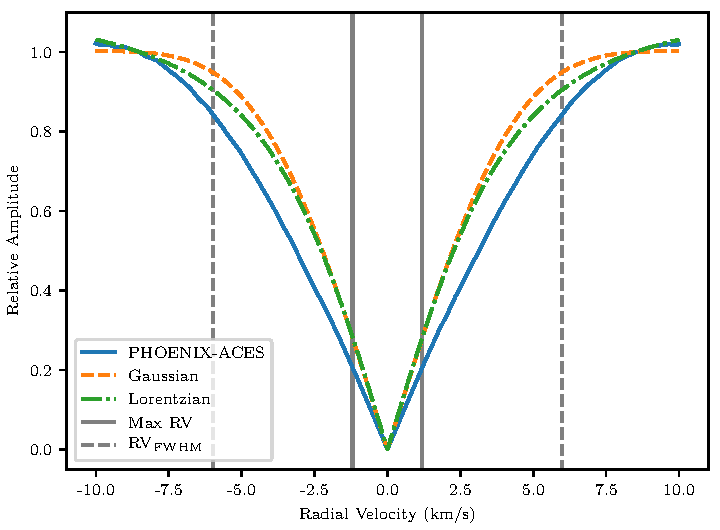
\includegraphics[width=0.45\textwidth]{figures/direct-recovery/rv_diff_final.pdf}
	\caption{Simulated relative amplitude of differential spectra at different RV separations revealing the diminished amplitude at small orbital separations. The solid blue line shows the maximum relative amplitude of the differential signal (from a shifted copy of itself) of a PHOENIX-ACES spectrum with \(T_{\textrm{eff}}=2500~K, logg=5.0, [Fe/H]=0.0\) in the wavelength region 2110--2123~nm. The maximum difference is normalized by the average amplitude between 7--10\kmps{}, representing a complete line separation. The orange (dashed) and green (dot-dashed) lines represent the relative amplitude of a differential spectrum of a spectrum containing a single Gaussian and single Lorentzian absorption line respectively, each with a unitary amplitude and a \(\rm FWHM = \lambda / R\). Beyond the FWHM lines the difference of the synthetic spectrum becomes more complicated due to the interaction of neighbouring lines. The solid vertical lines indicate the estimated companion \(\Delta RV\) in these observations while the dashed vertical lines indicate the RV corresponding to the FWHM at this wavelength and resolution. Beyond the FWHM RV the synthetic spectrum becomes complicated due to the interaction of neighbouring lines.}

	\label{fig:diff_amp}
\end{figure}
\unfinished{Increase size of diff amp plots to two}

\unfinished{Try show differences for all targets /all chips?}



\section{Estimating Companion-host Flux ratio}

\unfinished{Move location / adjust from paper}
\label{compaion flux ration}
The companion-host flux or contrast ratio of the systems are calculated using \( \frac{F_{2}}{F_{1}} \approx 2.512^{m_{1}-m_{2}} \), where \(m_{1}\) and \(m_{2}\) are the magnitude of the host and companion respectively.\ \(m_{1}\) is the magnitude of the host in the literature, while \(m_{2}\) is obtained from stellar evolution models of~\citet{baraffe_evolutionary_2003, baraffe_new_2015}, using the companion mass (or \(M_{2}\sin{i}\))) and the host's age. If only the companion minimum mass is known then this will correspond to the flux ratio lower limit, (or worst case scenario). The models, interpolated to the companion mass, also provide a first estimate of companion properties such as \(T_{\textrm{eff}}\), logg, \(R/R_{\sun}\) and the magnitude in many wavelength bands.
We use the K-band magnitude specifically for this work to estimate the flux ratio between the host and companion using the host K-band magnitude obtained from SIMBAD~\citep{wenger_simbad_2000}. Our flux ratio estimates are presented in table~\ref{tab:flux_table}.
The companion \(T_{\textrm{eff}}\) and logg values specifically are used to influence the selection of synthetic model grids to perform the \(\chi^2\) analysis over.

\subsection{baraffe tables}
A simple tool\footnote{Available at \url{https://github.com/jason-neal/baraffe_tables}} was created to estimate the host-companion flux ratio using the~\citep{baraffe_evolutionary_2003,baraffe_new_2015} evolution tables. The minimum requirements are the host star name, the companion mass and a stellar/system age. The host's name is used to query the SIMBAD database to obtain available stellar properties, specifically for this work the photometric \textit{K}-band magnitudes and parallax. There are several Baraffe tables for different stellar ages. If the age given does not correspond to a published table then interpolation between two tables is preformed. The table selected is interpolated to the companion mass provided and the entries returned.

There is also a script available which operates in reverse. Given a host name, age, and a flux ratio it will find the table position and corresponding companion mass that It can also work in reverse to estimate the companion mass when provided with a flux ratio value.




\section{Direct recovery in the MIR}
Early on in 2015 we began investigating extending this technique to the MIR. In particular looked at applying for observing time with a MIR instrument to perform a similar differential subtraction technique.
There were two reasons for this, to explore the MIR where the contrast ratios are higher and because we were unaware of high-resolution \nir{} instrument available, as CRIRES was being upgraded to CRIRES+.

We explored the use of VISIR to detect brown dwarf companions in the MIR. Of the targets in the correct location XXX was deemed to be the best case.

Looking at the best candidates XXXX was chosen a a likely target. I calculated flux ratios and performance considerations we determined that observations with VISIR to achieve a SNR of 100 were unfeasible, requiring 1000's of hours observing time.

The goal would be to observe with High-resolution and high through-put spectrographs. Ideally with CRIRES+, which at the time was scheduled for 2017. Currently\footnote{June 2018} first light is scheduled for Q1 2019.




\subsubsection{Differential scheduling challenges {copy from paper}}
\label{subsubsec:differential-schedualing}
This work has revealed that more care needs to be taken in planning the observations for the spectral differential analysis of faint companions in the future. Paying attention in particular to the FWHM of the lines in the region (governed by resolution and wavelength); the estimated companion \(\Delta RV \); the previous observations from different observing periods; and keeping consistent detector settings.

The original goal for the observations was to obtain two different and ``clearly separated radial-velocities'' for the secondary companion. However, the program was assigned a low-priority (C, in ESO grading) and, possibly due to operational reasons, the original time requirements necessary to secure well separated RVs for the companion spectra could not be met. This meant that all observations were insufficiently separated to extract a differential spectra for the companion.

The long orbital periods of these targets is also a contributing factor to the insufficient separations. Most of the targets observed here have orbital periods much longer than an observing semester (183 days). An optimal pair of observations (achieved at the extrema) would need to have been obtained from separate observing periods (between 2 months and 19 years apart). In some cases, even observations taken at the beginning and end of the semester would not be sufficient to achieve companion separation (depending on the phase). Requiring separate observing periods to even achieve the minimum \(\Delta \rm RV\) larger than the line FHWM.\@At the time it was impossible to ask for time over several semesters in a regular proposal.

Our study demonstrates the importance of proposals for projects that need to be extended over several semesters or years. In the ESO context, this corresponds to ``Monitoring proposals''~\citep[e.g.][pg. 18]{eso_eso_2017}. Observations of the targets explored here, with long orbital periods in particular, would benefit from the ability for multi-period proposals and newer scheduling systems which allow for tighter scheduling constraints, such as a companion RV separation.

For future observations we suggest that the known orbital solution of the companion be used to estimate the companions' RV curve during the observing period, with the companion \(M_2\sin{i}\) providing an RV upper-limit. Knowing the instrumental wavelength and resolution, a constraint can then be set to avoid taking observations when the companion spectra are insufficiently separated, or \(\Delta RV\) < FWHM.\@This constraint can be set using the absolute and relative \emph{time-link} constraints available in ESO's Phase 2 Proposal Preparation (P2PP) tool.
Additionally, analysing the known orbital solution before-hand, to determine RV constraints will also help identify the best time to observe, if observations from separate periods will be required or, if an optimally separated companion differential is even feasible.





\section{JUNK}


% from draft of paper 18/7/2017
\subsection{Companion K}
\label{sec:companion_RV}
\emph{These sections might be unnecessary}\\

To calculate the RV of the companion at the time of each observation. For a two-body system the RV semi-amplitude of the companion $\textrm{K}_{2}$ can be determined from the orbital host-companion mass ratio $q = \textrm{M}_{1}/\textrm{M}_{2} = \textrm{K}_{2}/\textrm{K}_{1}$.
Note, that for the targets in which only the minimum mass (msini) is known, this will give the maximum RV semi-amplitude of the companion.
This relation was used to estimate $\textrm{K}_2$ for the companion from the minimum mass or mass we have for each companion. These values along with the other orbital parameters of the system were use to calculate the RV of the companions for each observation. These values are provided with the observations in Table~\ref{tab:observations}.


\subsection{Companion-host Flux ratio}
The companion-host flux or contrast ratio of the systems are calculated using $ \frac{F_{2}}{F_{1}} \approx 2.512^{m_1-m_2} $, where $m_1$ and $m_2$ are the magnitude of the host and companion respectively.\ $m_1$ is the observed magnitude of the host while $m_2$ is obtained from stellar evolution models of~\citet{baraffe_evolutionary_2003, baraffe_new_2015}, using the companion mass or minimum mass and the host age. The models, interpolated to the companion mass, also provide a first estimate of companion properties such as $T_{eff}$, $R/R_{\odot}$ and the magnitude in many wavelength bands.
We use the K band magnitude specifically for this work to estimate the flux ratio between the host and companion using and the host K band magnitude obtained from SIMBAD~\citep{wenger_simbad_2000}. Our flux ratio estimates are presented in table~\ref{tab:estimated_fluxratio}.

If only the companion minimum mass is known then this will correspond to the flux ratio lower limit, (or worst case scenario).


A simple tool to do this calculation was created with python. Given a host name, companion mass and a stellar age it can give a flux contrast ratio of the system. A script to work backwards from a flux-ratio to a companion mass was also created as a check for the results from \S~ref$ {subsec:companion_recovery}$. These scripts can be found at \url{https://github.com/jason-neal/baraffe_tables}.




TAPAS XML REQUESTER

Although TAPAS provides a convenient web-interface to retrieve telluric spectra, it is tedious to use when requesting many models. A script\footnote{Can be found at \url{github.com/separate repo}} was used to automatically fill-out the XML template provided by TAPAS directly from values in the header information of each observation. Although created for these CRIRES observations it could be adjusted to work with other instruments if many TAPAS spectra are required. \textbf{It can be found at \ldots. Make separate Github repo for TAPAS requests.}


%!TEX root = ../thesis.tex
\begin{table*}
	\centering
	\small
	\caption{Stellar parameters of the target companion's host stars.}
		\begin{tabular}{l c c r@{$~\pm~$}l r@{$~\pm~$}l r@{$~\pm~$}l r@{$~\pm~$}l r@{$~\pm~$}l c}
		\toprule
		Star & SpT & V &  \multicolumn{2}{c}{\(T_{\textrm{eff}}\) (K)} &  \multicolumn{2}{c}{logg (cm s\(^{-2} \))} & \multicolumn{2}{c}{[Fe/H]} &  \multicolumn{2}{c}{\(M_1\) (M\(_{\sun} \))} & \multicolumn{2}{c}{Age (Gyr)} & Reference\\
		\midrule
        \object{HD 4747}     & K0V & 7.15 & 5316 & 50 & 4.48 & 0.10  & $-$0.21 & 0.05 & 0.81 & 0.02  & 3.3   & 2.3 & 1, 2, 3\\ 
		\object{HD 162020} & K3V & 9.12 & 4723 & 71 & 4.31 & 0.18  & $-$0.10 & 0.03 & 0.74 & 0.07  & 3.1   & 2.7 & 4, 5    \\  
		\object{HD 167665} & F9V & 6.48 & 6224 & 50 & 4.44 & 0.10  & 0.05       & 0.06 & 1.14 & 0.03  & 0.7   & 3.6 & 1        \\
		\object{HD 168443} & G6V & 6.92 & 5617 & 35 & 4.22 & 0.05 & 0.06       & 0.05 & 1.01 & 0.07  & 10.0 & 0.3 & 5, 6    \\ 
		\object{HD 202206} & G6V & 8.07 & 5757 & 25 & 4.47 & 0.03 & 0.29       & 0.02 & 1.04 & 0.07  & 2.9   & 1.0 & 5, 7    \\ 
		\object{HD 211847} & G5V & 8.62 & 5715 & 24 & 4.49 & 0.05  & $-$0.08 & 0.02 & 0.92 & 0.07  & 0.1   & 6.0 & 2, 4    \\ 
		\object{HD 30501}   & K2V & 7.59  & 5223 & 50 & 4.56 & 0.10 & 0.06       & 0.06 & 0.81 & 0.02  & 0.8   & 7.0 & 1, 4    \\ 
		\bottomrule
	\end{tabular} \\
	\tablebib{
	          (1) \citet{sahlmann_search_2011}; (2) \citet{santos_spectroscopic_2005}; (3) \citet{crepp_trends_2016}; (4) \citet{tsantaki_deriving_2013}; (5) \cite{bonfanti_age_2016}; (6) \citet{santos_spectroscopic_2004};
	          (7) \citet{sousa_spectroscopic_2008};
	          }
	\label{tab:starparams}
\end{table*}
%!TEX root = ../thesis.tex
% Table of orbit parameters

\todo{Rotate orbital parameter table.}
\begin{table*}
		\centering
		\tiny
		\caption{Orbital parameters for the BD companions obtained from the literature.}
		\begin{tabular}{l c r@{$ \,\pm\, $}l r@{$ \,\pm\, $}l r@{$ \,\pm\, $}l r@{$ \,\pm\, $}l r@{$ \,\pm\, $}l cc c c}
		\toprule
		Object  & \(\gamma \)  	& \multicolumn{2}{c}{Period}   & \multicolumn{2}{c}{\(e \) } &  \multicolumn{2}{c}{\(\textrm{K}_{1} \) } &  \multicolumn{2}{c}{\(T_{0} \)}  &  \multicolumn{2}{c}{ \(\omega \) } & \(M_2\sin{i}\) & \(M_2\) & Ref.\\
		 & (km\(^{-1} \)) 	& \multicolumn{2}{c}{(day)}   	&    \multicolumn{2}{c}{}    &  \multicolumn{2}{c}{(ms\(^{-1} \))}   & \multicolumn{2}{c}{ (JD-2,450,000) } &  \multicolumn{2}{c}{(deg) } &   \(\rm {M}_{Jup} \)  &   \(\rm {M}_{Jup} \)   & \\
		\midrule
		\object{HD 4747}       & $0.215 \pm 11 $        	 &  13826.2  &  314.1            &  0.740 & 0.002  	& 755.3   &  12      & 463.1       &  7.3    & 269.1      &  0.6   &  39.6    & 60.2 			  & 1 \\
		\object{HD 162020}   & $-27.328\pm0.002$  	    &  8.42819  &  $6e^{-5}$   &  0.277 & 0.002   & 1813    &  4        & 1990.68   &  0.01  & 28.4        &  0.2   & 14.4     &     -   			  & 2 \\
		\object{HD 167665}   & $8.003 \pm 0.008$    	 & 4451.8 & 27.6   				   & 0.340 & 0.005 	  & 609.5   &  3.3     & 6987.6     &  29     & $-$134.3 & 0.9     & 50.3    &     -    			& 3 \\
		\object{HD 168443}b  & $-0.047\pm0.552$ 		& 58.1124 & $4e^{-4}$  		& 0.529 & 0.001   & 475.13 & 0.9      & 5626.20  &  0.02   & 172.9      & 0.1     & 7.7      &     -    			& 4 \\ 
		\object{HD 168443}c  & $-0.047\pm0.552$ 		 & 1749.83 & 0.57  			     & 0.211 & 0.002  	 & 297.7  & 0.6      & 5521.3     &  2.2     & 64.9       & 0.5     & 17.1    &     -    			  & 4 \\ 
		\object{HD 202206}B & 14.721     						& 256.33  &  0.02    		     & 0.432 & 0.001  	  & 567     &  1       & 2176.14    &  0.12   & 161.9     & 0.2  	& 17.4    & $93.2\pm7.3$   & 5, 6\\  
		\object{HD 202206}c & 14.721    						 & 1260 &  11			        	& 0.22 & 0.03 		  & 41    	& 1          & 3103 		& 452    & 280 		   & 4  	  & 2.3      & $17.9\pm2.9$  & 5, 6\\ 
		\object{HD 211847} 	 & 6.689\tablefootmark{a} & 7929.4 & 2500  		    	 & 0.685 & 0.068   	  & 291.4   & 12.2   & 12030.1    & 2500   & 159.2 		& 2.0     & 19.2  & 155  				& 3, 7\\
		\object{HD 30501}  	  & $23.710\pm0.028$         & 2073.6 & 3.0 				& 0.741 & 0.004   	   & 1703.1 & 26.0   & 3851.5 		& 3.0     & 70.4 		& 0.7     & 62.3   & 89.6      			& 3  \\
		\bottomrule
	\end{tabular}
	\tablebib{
	          (1) \citet{crepp_trends_2016}; (2) \citet{udry_coralie_2002}; (3) \citet{sahlmann_search_2011}; 
	          (4) \citet{pilyavsky_search_2011}; (5) \citet{correia_coralie_2005};  (6) \citet{benedict_hd_2017}; (7) \citet{moutou_eccentricity_2017}
	}
	\tablefoot{
	\tablefoottext{a}{fixed}
	}
	\label{tab:orbitparams}
\end{table*}



CHECK out LOCKWOOD 2014 - maximum likelihood with todcor 1e-4 flux ratio double lined spectra